% This is a LaTeX thesis template for Monash University.
% to be used with Rmarkdown
% This template was produced by Rob Hyndman
% Version: 6 September 2016

\documentclass{monashthesis}

%%%%%%%%%%%%%%%%%%%%%%%%%%%%%%%%%%%%%%%%%%%%%%%%%%%%%%%%%%%%%%%
% Add any LaTeX packages and other preamble here if required
%%%%%%%%%%%%%%%%%%%%%%%%%%%%%%%%%%%%%%%%%%%%%%%%%%%%%%%%%%%%%%%

\author{Xiefei Li}
\title{Revisiting the forecast combination puzzle with different data types: An empirical study}
\studentid{30204232}
\studentemail{\href{mailto:xlii0145@student.monash.edu}{\nolinkurl{xlii0145@student.monash.edu}}}
\studentdetails{Supervisor: David T. Frazier}
\supervisoremail{\href{mailto:David.frazier@monash.edu}{\nolinkurl{David.frazier@monash.edu}}}
\def\degreetitle{Bachelor of Commerce (Honours)}
% Add subject and keywords below
\hypersetup{
     %pdfsubject={The Subject},
     %pdfkeywords={Some Keywords},
     pdfauthor={Xiefei Li},
     pdftitle={Revisiting the forecast combination puzzle with different data types: An empirical study},
     pdfproducer={Bookdown with LaTeX}
}


\bibliography{thesisrefs}

\begin{document}

\pagenumbering{roman}

\titlepage

{\setstretch{1.2}\sf\tighttoc\doublespacing}

\clearpage\pagenumbering{arabic}\setcounter{page}{1}

\hypertarget{introduction}{%
\chapter{Introduction}\label{introduction}}

\hypertarget{research-question-and-objective}{%
\section{Research Question and Objective}\label{research-question-and-objective}}

This \textbf{thesis aims to investigate} the \textbf{determinants behind, and evidence for,} the forecast combination puzzle in various settings, besides the time series domain, and to empirically examine a general solution to the forecast combination puzzle. The combination puzzle refers to the \textbf{well-known empirical finding that an equally weighted combination of forecasts generally} outperforms \textbf{more} sophisticated combination \textbf{schemes}. Over the past 50 years, the empirical study undertaken so far has been limited, in that most attention has been focused on different time series datasets. \textbf{Thus, one of the main contributions of this research will be to investigate the presence of the combination puzzle in settings outside of pure time series models. As an additional contribution, we will investigate the veracity, and applicability, of a recently proposed solution to forecasting combination puzzle suggested in \textcite{ZMFP22} and \textcite{FZMP23}.}

\hypertarget{motivation}{%
\section{Motivation}\label{motivation}}

\textbf{The accuracy of forecasts is of critical concern} when forecasts are used in decision-making. \emph{Under the classical frequentist approach, forecasters often choose only one ``best model'' to mimic the actual data generating process of the target variable and then use it to predict future values.} \textcolor{red}{This is not true in general. What you are doing is frequentist actually, so I also don't see the need to be distinct here. Perhaps best to say something instead about: one possible approach would be to choose a single best model and use the resulting model to produce our forecasts. However, that single model, even if chosen optimally, may not capture all important information about the data generaring process.} However, that single model could be misleading, as it may not capture all the important features of the data. The idea of combining multiple \textbf{forecasts from different models was originally proposed in the seminar work of } \textcite{BG69}. They popularized the use of forecast combination for optimal forecasts with several combination techniques. The dramatic improvements in forecast accuracy, along with flexible combination methods, have attracted increasing attention and contributions from researchers in different fields, both theoretical and empirical {[}\textcite{C89};T06{]}; see \textcite{WHLK22} for a modern literature review over the past 50 years.

In short, forecast \textbf{combination methods} involve producing point or density forecasts and then combining them based on a rule or weighting scheme. This process can \textbf{sometimes capture more meaningful features of the true data generating process than using a single model, and allows us to combine the best features of different models within a single framework}. \textcolor{red}{This makes it seem like you are saying the forecast puzzle is due to carelessness... which is a very bad idea. Best to revise this sentence or just describe the phenomena.} However, issues could arise with arbitrary or careless implementation. \textbf{IN most time series settings under which forecast combinatinos are employed, a striking empirical phenomena is often observed, coined by \textcite{SW04}, as the ``forecast combination puzzle''. The puzzle is the encapsulated by the fact that} ``theoretically sophisticated weighting schemes should provide more benefits than the simple average from forecast combination, while empirically the simple average has been continuously found to dominate more complicated approaches to combining forecasts'' \autocite{WHLK22} (see section 2.6 for more details and examples).

\textcolor{red}{Can't use this if you haven't said why it is counter-intuitive. Ask yourself, why is this counterintuivie? }
This counter-intuitive result is widely discovered in time series settings, what will happen when working with datasets such as surveys of professional forecasters, dynamic panels, and pure cross-sectional?

\textcolor{red}{you need a more extensive review here. Go back through the papers Wang et al. mentions in their review, as well as the other review I mentioned, and try and pick out several more key references to discuss. In particular, you also need to present some information on the various solutions for the puzzle that have so far been suggested, which is conspicuously missing; e.g., Smith and Wallis, The paper by Hjort and Vasney, etc. We weren't the first to present a solution, our solution is just the most general, and nests all the other proposed solutions}

\textcolor{red}{This can then be more carefully connected with the following paragraph}

\textbf{While various explanatinos for the forecast combination puzzle have been suggested over the years (see the above references), a general solution to the puzzle has so far proved ellusive.} If the forecast combination puzzle occurs in every setting, it is essential to explore its cause and support the theory with empirical evidence.
\textcolor{red}{These two ideas are far to disperate to be presented in the same paragraph. You need to pull them apart and make each a separate idea with their own paragraphs. They can't be so easily smushed together.}
\textcite{FZMP23} demonstrated that, in theory, the cause of the puzzle is the way researchers produce forecast combinations, called a ``two-step'' approach in the paper. The constituent model forecasts are determined first with estimated parameters, and the unknown weights are then estimated conditional on all the estimates. \textcolor{red}{Revise this, it is unclear what you are trying to say here or why. I think what you are trying to state is why people use the two-step approach in general. } Due to the unawareness and dimensionality of combining all unknown parameters, this two-step approach is commonly studied and used in the literature, e.g., \textcite{HM07}; \textcite{GA11}; \textcite{GR13}; \textcite{BS16}. \textcite{FZMP23} further claims that the forecast combination puzzle can be avoided when unknown parameters and weights are estimated in one step, namely a ``one-step'' approach, when feasible. In other words, if forecasts are produced by estimating parameters and weights simultaneously, the sophisticated weighting schemes should (asymptotically) be superior.

\textbf{The goal of this thesis is two-fold: first, to search for empirical evidence of the combination puzzle in settings outside of the ususal time series in which it has been found; second, to test the empirical veracity of the theoretical solution to the puzzle found in \textcite{FZMP23}, both within, and outside of, the standard time series setting where the puzzle is often observed.}
\textcolor{red}{There is no neet to talk about testing at this stage, as you can't scratch the surface of this idea yet, and placing it here looks awkward without the necessary literature to back it up}

\hypertarget{methodology}{%
\chapter{Methodology}\label{methodology}}

\textbf{The first} goal of this paper is to construct linear density forecast combinations with several potential parametric models of a dataset. In addition to point forecasts, the use of density forecasts can offer forecasters or decision markers a broader and more comprehensive view of the target variable (see section 2.6.1. of \textcite{FTP22} for related contributions). The two-step approach will be applied in this part, and the results are anticipated to reveal that forecast combinations can \textbf{deliver improved accuracy over single models, but are not necessarily superior to forecasts obtained from the equally weighted combination.}

The next goal is to estimate the unknown parameters of the constituent models and the weight in a single step, \textbf{and to compare the accuracy of forecasts based on these combinatinos against the usual (two-step) combinations, as well as the equally weighted combination. To measure differences between these forecasts, we will eventually employ forecast accuracy tests, which measure out-of-sample differences between forecasts.}
\textcolor{red}{You need to give some references for such tests if you are going to present them. There are a plethora going back to Diebold and Mariano, White (2000), Giacomini and White (2000), West (1996). Just see the references in our paper}

Before further explaining the details, the following notations will be used throughout the paper. The dataset with \(T\) observations will be divided proportionally into two parts, an in-sample period \(R\) and an out-of-sample period \(P\). The realization of a target variable \(y\) at time \(t\) is denoted as \(y_{t}\). Its future value after the in-sample period is denoted as \(y_{\small{R+h}}\), where \(h\) is the forecast horizon. \(\mathcal{F}_t\), the information set at time t, is comprised of all observed (and known) realizations of \(y\) up to time t, i.e., \(\mathcal{F}_t = \{y_1, y_2, .., y_t\}\).

\hypertarget{forecast-combination-method}{%
\section{Forecast Combination Method}\label{forecast-combination-method}}

\textcolor{red}{You need much more detail here. At a minimum you need to more clearly define: 1) the parameters in the constituent models; 2) what you mean by the MLE; how you're estimating the combination weight in (2.1)}
For the first step, I will estimate the unknown parameters of each constituent model using Maximum Likelihood Estimation. These estimates will then be held fixed and substituted into their corresponding probability density functions.

Based on the idea of linear pooling \autocite{BG69,HM07,GA11}, the linear combinations of two predictive densities \(f^{(t)}\) will be constructed with two constituent predictive densities \(f^{(t)}_1\) and \(f^{(t)}_2\):

\begin{equation}
f^{(t)}(y) = wf^{(t)}_1(y) + (1-w)f^{(t)}_2(y)
\end{equation}\\
\textcolor{red}{This is not generally necessary, and is only what you do in the empirical section. you can leave these as general models for now.}
where \(f^{(t)}_1(y)\) and \(f^{(t)}_2(y)\) are assumed to follow the normal distributions but with different means and variances, \(h\) is the future value after the in-sample period (\(R\)), and \(w\) is the weight allocated to the first model. Through this construction, the sum of two weights is implied to be 1, which is necessary and sufficient for the combination to be a density function\autocite{GA11}.

More specifically, \(f^{(t)}_1(y)=f_1(y_t|\mathcal{F}_{t-1})=N\{y_t; \mu_1, \sigma^2_1\}\) and \(f^{(t)}_2(y)=f_2(y_t|\mathcal{F}_{t-1})=N\{y_t; \mu_2, \sigma^2_2\}\). \(N\{x; \mu, \sigma^2\}\) denotes the normal probability density function evaluated at value \(x\) with mean \(\mu\) and variance \(\sigma^2\). Given \(\mathcal{F}_{t-1}\), the conditional mean and conditional variance should be used.

\textcolor{red}{The estimation steps should all be in the same section, not split across two as you have it now.}

\hypertarget{evaluation}{%
\section{Evaluation of Models and Weighted Forecast Combinations}\label{evaluation}}

This refers to the second step, where I estimate the weight that is assigned to the first model given the aforementioned estimates. The assessment of out-of-sample predictions for individual models and combinations will rely on the average log predictive score function.

The average log predictive score function of a specific model over the forecast horizon \(h=1,2,...,P\) (i.e., the out-of-sample period) is defined as follows:

\begin{equation}
LS = \frac{1}{P}\sum^P_{h=1}logf(y_{\small{R+h}}) = \frac{1}{P}\sum^P_{h=1} logf(y_{\small{R+h}}| \mathcal{F}_{\small{R+h-1}})
\end{equation}

\textbf{The optimal weight \(w*\) } \textcolor{red}{This is not correct. We estimate the weights and the combinatinos on the same sample, then take them both out of sample according to equation (2.1)} will be estimated by maximizing the average logarithmic predictive score function over the out-of-sample period:

\begin{equation}
\frac{1}{P}\sum^P_{h=1}log\Big[wf_1(y_{\small{R+h}}|\mathcal{F}_{\small{R+h-1}}) + (1-w)f_2(y_{\small{R+h}}|\mathcal{F}_{\small{R+h-1}})\Big]
\end{equation}

The corresponding forecast density combination, given the optimal weight, will be referred to as the optimal combination.

\textbf{Why are we using this \(LS\), and what does it buy us? How does this help us look at the accuracy of density forecasts? These questions need to be answered here\ldots{}}

\hypertarget{a-motivating-example}{%
\section{A Motivating Example}\label{a-motivating-example}}

\hypertarget{data}{%
\subsection{Data}\label{data}}

Reconsidering the example in section 3 of \textcite{GA11}, I use the daily Standard and Poor's (S\&P) 500 index from February 11, 2013 to February 10, 2023 (10 years in total), retrieved via the \textcite{SP500}. Total 2519 (\(T\)) available observations are partitioned into two periods with a rough proportion. The in-sample period contains the first 60\% of the data (\(R = 1511\)), which is used for estimating unknown parameters in each model. The remaining 40\% (\(P = 1008\)) becomes the out-of-sample period for further evaluation.

\hypertarget{model}{%
\subsection{Model Specification}\label{model}}

For simplicity, I use five prediction models to study the performance of two-model pools:

\begin{enumerate}
\def\labelenumi{\arabic{enumi}.}
\tightlist
\item
  Model 1: An ARIMA(1,1,1) model with an intercept for the natural logarithm of S\&P 500.
\item
  Model 2: An ETS(M,N,N) model for the S\&P 500.
\item
  Model 3: An ETS(M,A,N) model for the S\&P 500.
\end{enumerate}

ARIMA is short for autoregressive integrated moving average, and ETS stands for exponential smoothing. All error terms are assumed to be independent and normally distributed with mean zero and variance \(\sigma_m^2 \ \text{for}\  m = 1,2,3\).

\begin{enumerate}
\def\labelenumi{\arabic{enumi}.}
\setcounter{enumi}{3}
\tightlist
\item
  Model 4: A linear regression model for the S\&P 500 with a trend regressor and errors, follow an ARIMA(1,0,0) process.
\item
  Model 5: A linear regression model for the natural logarithm of S\&P 500 with a trend regressor and errors follow an ARIMA(1,0,0) process.
\end{enumerate}

Both error terms in the ARIMA model are assumed to be independent and normally distributed with mean zero and variance \(\sigma_m^2 \ \text{for}\  m = 4,5\).

All unknown parameters are estimated by maximizing the likelihood function using the in-sample period data. Once the estimated are obtained, they are held fixed for the density evaluations. For each model, I generate the predictive densities at every future time point of S\&P 500 returns (\(h=1,2,...,P\)) given that all past information is known. In order to make a comparison between each pair of these models, the log of S\&P 500 returns will be ``back-transformed'' by evaluating with the log normal density function.

As a reference, detailed formulas and explanations of these models can be found in \textcite{fpp3}. The formula of the conditional variance for the ETS models in this case is discussed in Chapter 6.3 of \textcite{HKOS08}. All coding is performed using R Statistical Software (version 4.2.1 (2022-06-23)). The packages used are \texttt{tidyverse} \autocite{tidy19}, \texttt{dplyr} \autocite{dplyr23}, and \texttt{fpp3} \autocite{fpp23}.

\hypertarget{preliminary-results}{%
\chapter{Preliminary Results}\label{preliminary-results}}

The average log predictive score of each model mentioned in section \ref{model} is calculated and presented in Table \ref{tab:1}. If only one model can be chosen, the model with the highest score will be preferred, which is the ETS(M,A,N) model with a score of -5.8351 in this case. The differences among models seem to be small, disregarding the linear model on the level of S\&P 500 returns, but they are closely related to the number of out-of-sample observations and the effect of natural logarithm. Taking these into consideration, the ETS(M,A,N) model could be strongly favored.

\vspace{0.3cm}

\begin{table}[htbp!]
\centering
\caption{Average log predictive score of each proposed model for S\&P 500 returns.}
\begin{tabular}{l*{4}{c}cccccccc}
\hline
     ARIMA(1,1,1) & ETS(M,N,N) & ETS(M,A,N) & LM (linear) & LM (log) \\
    \hline
     -5.8643 & -5.8373  & -5.8351 & -7.4724 & -5.8716\\
    \hline
\end{tabular}
\label{tab:1}
\end{table}

\vspace{0.3cm}

Besides, there are 10 pairs of two-model combinations given 5 models. For each combination, I generated all the average log predictive scores when the weight on the first model in that combination increases from 0 to 1 by a 0.01 change every time. The optimal combination is generated according to section \ref{evaluation}. Table \ref{tab:2} presents the information about the optimal combination of every pair, including the highest log score and the optimal weight.

\vspace{0.3cm}

\begin{table}[htbp!]
  \centering
  \caption{Average log predictive score of density forecasts combination under two-model pools}
    \begin{tabular}{llllll}
    \toprule
          & ARIMA(1,1,1) & ETS(M,N,N) & ETS(M,A,N) &  LM (linear) &  LM (log) \\
    \midrule
    ARIMA(1,1,1) & \textit{-5.8643} & -5.793 & -5.7964 & -5.8643 & -5.8473 \\
    ETS(M,N,N) & 0.45  & \textit{-5.8373} & -5.8351 & -5.8373 & -5.8121 \\
    ETS(M,A,N) & 0.43  & 0.08  & \textit{-5.8351} & -5.8351 & -5.8133 \\
     LM (linear) & 1     & 1     & 1     & \textit{-7.4724} & -5.8716 \\
     LM (log) & 0.56  & 0.65  & 0.67  & 0     & -5.8716 \\
    \bottomrule
    \multicolumn{6}{l}{\footnotesize The diagonal entries contains individual average log scores for each model.}\\
    \multicolumn{6}{l}{\footnotesize The highest average log scores for optimal pools are located above the diagonal.}\\
    \multicolumn{6}{l}{\footnotesize Entries below the diagonal show the optimal weight of the model in that column in the two-model pool.}\\
    \end{tabular}
  \label{tab:2}
\end{table}

\vspace{0.3cm}

More specifically, I picked the first 4 highest score as shown in Table \ref{tab:3}.

\vspace{0.3cm}

\begin{table}[htbp!]
  \centering
  \caption{The best four density forecasts combinations evaluated by the average log predictive score}
    \begin{tabular}{ll}
    \toprule
    Combination & Average log predictive score \\
    \midrule
    ARIMA(1,1,1) \& ETS(M,N,N) & -5.793 \\
    ARIMA(1,1,1) \& ETS(M,A,N) & -5.7964 \\
    ETS(M,N,N) \&  LM (log) & -5.8121 \\
    ETS(M,A,N) \&  LM (log) & -5.8133 \\
    \bottomrule
    \end{tabular}
  \label{tab:3}
\end{table}

\vspace{0.3cm}

The Figure \ref{fig:best4} illustrates the changes in the average log predictive score as the weight increases for the best 4 combinations.

\vspace{0.3cm}

\begin{figure}[htbp!]
\centering
\caption{The highest four average log predictive scores of weighted two-model-pool combinations for S\&P 500 returns predictive densities. }
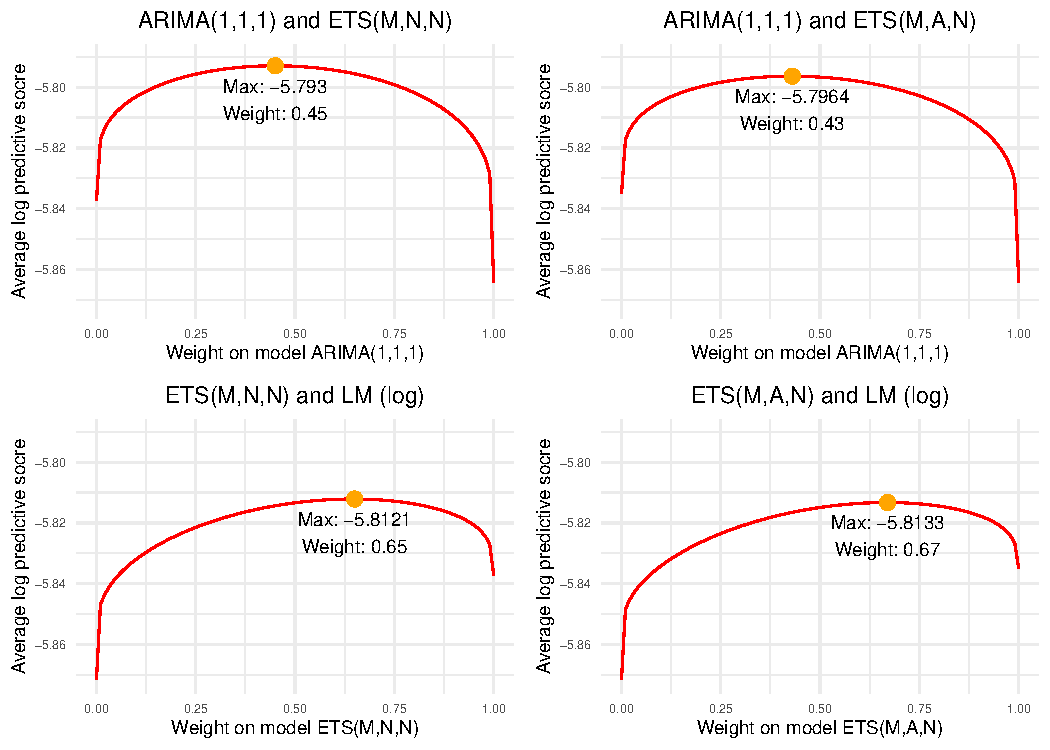
\includegraphics{figures/best4.pdf}
\begin{flushleft}
{\footnotesize The weights on the first model is in the x-axis and the corresponding average log predictive scores are on the y-axis. Constitutent models are stated in the title. The orange point represent the highest average log score of a specific combination. Its value and the corresponding optimal weight are noted below.}\\
\end{flushleft}
\label{fig:best4}
\end{figure}

\appendix

\hypertarget{appendix}{%
\chapter{Appendix}\label{appendix}}

All analyses were performed using R Statistical Software (R version 4.2.1 (2022-06-23))

Packages used are \texttt{tidyverse} \autocite{tidy19}, \texttt{dplyr} \autocite{dplyr23}, and \texttt{fpp3} \autocite{fpp23}.

\[\begin{aligned}
M_1: log(y_t) &= \phi_{0,1} + log(y_{t-1}) + \phi_{1,1}log(y)_{t-1} + \theta_{1,1}\epsilon_{t-1} + \epsilon_{t,1} \ \ \ \ \epsilon_t \stackrel{i.i.d.}{\sim} N(0,\sigma_1^2) \\
M_2: y_t &= \ell_{t-1,2}(1+\epsilon_{t,2}) \\
  \ell_{t,2} &= \ell_{t-1,2}(1+\alpha_2\epsilon_{t,2}) \\
M_3: y_t &= (\ell_{t-1}+b_{t-1}) (1+\epsilon_{t,3}) \\
  \ell_t &= \ell_{t-1}(1+\alpha\epsilon_{t,2}) \\
M_4&: y_t = \\
M_5&: y_t = 
\end{aligned}\]

\begin{equation}
  y_t - y_{t-4} = \beta (x_t-x_{t-4}) + \gamma (z_t-z_{t-4}) + \phi_1 (y_{t-1} - y_{t-5}) + \Theta_1 \varepsilon_{t-4} + \varepsilon_t
\end{equation}

\textcite{fpp3}

\printbibliography[title={Reference}]




\end{document}
